% VLDB template version of 2020-08-03 enhances the ACM template, version 1.7.0:
% https://www.acm.org/publications/proceedings-template
% The ACM Latex guide provides further information about the ACM template

\documentclass[sigconf, nonacm]{acmart}

\usepackage{amsmath}
\usepackage{amsthm}
\usepackage{amsfonts}
\usepackage[linesnumbered,ruled,vlined]{algorithm2e}
\usepackage{xspace}
\usepackage{xcolor}
\usepackage{enumitem}
\usepackage{array}
\usepackage{stmaryrd}
\usepackage{graphicx}
\usepackage{float}
\usepackage{pifont}
\usepackage{listings}
\usepackage{subcaption}
\usepackage{multicol}
\usepackage{multirow}

\newtheorem{theorem}{Theorem}
\newtheorem{example}{Example}
%% The following content must be adapted for the final version
% paper-specific
\newcommand\vldbdoi{XX.XX/XXX.XX}
\newcommand\vldbpages{XXX-XXX}
% issue-specific
\newcommand\vldbvolume{14}
\newcommand\vldbissue{1}
\newcommand\vldbyear{2020}
% should be fine as it is
\newcommand\vldbauthors{\authors}
\newcommand\vldbtitle{\shorttitle} 
% leave empty if no availability url should be set
\newcommand\vldbavailabilityurl{URL_TO_YOUR_ARTIFACTS}
% whether page numbers should be shown or not, use 'plain' for review versions, 'empty' for camera ready
\newcommand\vldbpagestyle{plain} 


\def\ojoin{\setbox0=\hbox{$\bowtie$}%
  \rule[-.02ex]{.25em}{.4pt}\llap{\rule[\ht0]{.25em}{.4pt}}}
\def\leftouterjoin{\mathbin{\ojoin\mkern-5.8mu\bowtie}}
\def\rightouterjoin{\mathbin{\bowtie\mkern-5.8mu\ojoin}}
\def\fullouterjoin{\mathbin{\ojoin\mkern-5.8mu\bowtie\mkern-5.8mu\ojoin}}

\newcommand{\kw}[1]{{\ensuremath {\mathsf{#1}}}\xspace}
\newcommand{\kws}[1]{\textsf{\scriptsize{#1}}\xspace}
\newcommand{\bkw}[1]{{\ensuremath {\mathsf{\textbf{#1}}}}\xspace}

\newcommand{\kwnospace}[1]{{\ensuremath {\mathsf{#1}}}}
%=============defined for reference======
\newcommand{\attr}{\kw{attr}}
\newcommand{\sch}{\kw{sch}}
\newcommand{\Dom}{\kw{Dom}}
\newcommand{\meta}{\kw{meta}}
\newcommand{\vars}{\kw{vars}}
\newcommand{\vlabel}{\mathcal{L}}
\newcommand{\elabel}{\mathcal{T}}
\newcommand{\lab}{\kw{Label}}
\newcommand{\type}{\kw{Type}}
\newcommand{\labx}{\kwnospace{Label}}
\newcommand{\id}{\kw{Id}}
\newcommand{\idx}{\kwnospace{Id}}
\newcommand{\shortest}{\kw{min}}
\newcommand{\simple}{\kw{simple}}
\newcommand{\pred}{\kw{pred}}
\newcommand{\vpred}{\kw{vpred}}
\newcommand{\epred}{\kw{epred}}
\newcommand{\getV}{\kw{getV}}
\newcommand{\getE}{\kw{getE}}
\newcommand{\short}{\kw{short}}
\newcommand{\In}{\downarrow}
\newcommand{\Out}{\uparrow}
\newcommand{\Both}{\updownarrow}
\newcommand{\InE}{\swarrow}
\newcommand{\OutE}{\nearrow}
\newcommand{\BothE}{\neswarrow}
\newcommand{\NotIn}{\bar{\In}}
\newcommand{\NotOut}{\bar{\Out}}
\newcommand{\NotBoth}{\bar{\Both}}
\newcommand{\vecExpandIn}{\vec{\In}}
\newcommand{\vecExpandOut}{\vec{\Out}}
\newcommand{\vecExpandBoth}{\vec{\Both}}
\newcommand{\allDistinct}{\not\equiv}
\newcommand{\params}{\kw{params}}
\newcommand{\code}{\texttt}
\newcommand{\apply}{\mathcal{A}}
\newcommand{\segapply}{\mathcal{SA}}
% enclose given text with a single quote in the math mode
\newcommand{\sq}[1]{`#1\mrq}
\newcommand{\either}{\kw{Either}}
\newcommand{\todo}[1]{\textcolor{red}{$\Rightarrow$#1}}


\begin{document}
\title{Converged Optimizer for Efficient Join Order Optimization}

%%
%% The "author" command and its associated commands are used to define the authors and their affiliations.
%\author{Ben Trovato}
%\affiliation{%
%  \institution{Institute for Clarity in Documentation}
%  \streetaddress{P.O. Box 1212}
%  \city{Dublin}
%  \state{Ireland}
%  \postcode{43017-6221}
%}
%\email{trovato@corporation.com}


\begin{abstract}
\revisewy{The recent ISO SQL:2023 standard adopts SQL/PGQ (Property Graph Queries), facilitating graph-like querying within relational databases. This advancement, however, underscores a significant gap in how to effectively optimize SQL/PGQ queries within relational database systems. To address this gap, we extend the foundational} \spj (Select-Project-Join) queries to \spjm queries, which include an additional matching operator for representing graph pattern matching in SQL/PGQ. Although \spjm queries can be converted to \spj queries and optimized using existing relational query optimizers, our analysis shows that such a graph-agnostic method fails to benefit from graph-specific optimization techniques found in the literature. To address this issue, we develop a converged relational-graph optimization framework called \name for optimizing \spjm queries, leveraging joint efforts from both relational and graph query optimizations. Using DuckDB as the underlying relational execution engine, our experiments show that \name can generate efficient execution plans for \spjm queries. On well-established benchmarks, these plans exhibit an average speedup of $14.72\times$ compared to those produced by the graph-agnostic optimizer.
    %Besides, experimental results on micro benchmarks illustrate the efficiency of the proposed optimization strategies.
    %Additionally, experimental results from micro-benchmarks demonstrate the effectiveness of the optimization strategies. In particular, by applying constraints directly within the matching operators, our approach achieves an improvement of up to 600 times. Moreover, eliminating fusion or using \texttt{expandintersect} can at least double the execution time of the generated plans.
    %Besides, the experimental results of ablation studies illustrate the efficiency of \expandintersect.
\end{abstract}


\maketitle

\section{Introduction}

SQL/Property Graph Queries (abbr.~SQL/PGQ) is Part 16 of SQL 2023, which has endowed traditional SQL with the ability to define and query graphs on top of relational databases.
In SQL/PGQ, Graphs are presented as views, and the vertices and edges in the graphs are represented as tables.
Please note that with SQL/PGQ, graph queries and relational queries can be expressed in one statement and optimized together for a better execution plan.
An example of a SQL/PGQ query is provided in Example \ref{example:introduction:sqlpgq}.

\begin{example}
    \label{example:introduction:sqlpgq}
    In this example, three tables, i.e., \textbf{Person, Knows, Department}, are stored in the relational database.
    With SQL/PGQ, a graph view named \textbf{friendship\_graph} is created based on tables \textbf{Person} and \textbf{Knows}.
    Specifically, rows in table \textbf{Person} represent the vertices in the graph while rows in table \textbf{Knows} represent the edges.
    Besides, the department a person belonging to is stored in table \textbf{Person} as a foreign key (\textit{dept\_id}).

    Suppose we are going to find three persons satisfying: (1) They know each other; (2) Two of them belong to the Department of Computer Science.
    Then, the corresponding SQL/PGQ query is as follows:
    \begin{equation}
        \begin{split}
            & \text{SELECT person1, person2, person3} \\
            & \text{FROM Department p, GRAPH\_TABLE (friendship\_graph} \\
            &            \hspace{2em} \text{MATCH} \\
            &            \hspace{3em} \text{(p1:Person)-[:Knows]-(p2:Person)-[:Knows]-(p3:Person),} \\
            &            \hspace{3em} \text{(p1)-[:Knows]-(p3)} \\
            &            \hspace{2em} \text{\text{COLUMNS} (} \\
            &                    \hspace{3em} \text{p1.name as person1,} \\
            &                    \hspace{3em} \text{p1.dept\_id as dept1,} \\            
            &                    \hspace{3em} \text{p2.name as person2,} \\
            &                    \hspace{3em} \text{p2.dept\_id as dept2,} \\ 
            &                    \hspace{3em} \text{p3.name as person3,}  \\
            &                    \hspace{3em} \text{p3.dept\_id as dept3,}  \\
            &        \hspace{2em} \text{)} \\
            & \text{WHERE} \\
            & \hspace{1em} \text{dept1 = p.dept\_id AND} \\
            & \hspace{1em} \text{dept2 = p.dept\_id AND} \\
            & \hspace{1em} \text{p.dept\_name = `\text{Computer Science}';} \\
        \end{split}
    \end{equation}

    According to the first condition, the wanted three persons should form a triangle in \textbf{friendship\_graph}.
    It is a problem of pattern matching, and such triangles are searched for on the graph view.
    The output of the graph query is a table (named f) with three columns, i.e., person1, person2, and person3, representing the identifiers of the three persons, respectively.

    For the second condition, due to the existence of the foreign key, it is efficient to perform natural join between table f and table \textbf{Department} to obtain the ideal results.
    Please note that the results of graph queries in SQL/PGQ are still tables, and such returned tables can be exploited in relational queries.
\end{example}

Query optimization is crucial for query processing.
The optimizer can significantly influence the efficiency of query processing.
There are already many works about relational query optimizers, and some works about graph query optimizers.
However, neither of them are suitable for SQL/PGQ queries.
Because they can only optimize the queries from the relational perspective or the graph perspective, but not both.
In this paper, we are going to propose a new converged framework for query optimization of SQL/PGQ statements.

There are mainly three challenges.

\textbf{Challenge 1. Relational optimizers cannot be used to optimize graph queries directly (or with limited efficiency)}.
It is true that the vertices and edges in graphs can be represented as corresponding tables in relational databases, and the paths in the graphs can be translated into join operators in relational algebra.
However, since the relational optimizers only take the relational operators into consideration, some efficient graph operators (e.g., get edge, get vertex, get neighbors with graph indices) are ignored in the process of optimization.
Therefore, the search space is artificially reduced, the best physical plan are likely to be missed.
An intuitive idea is to replace some relational operators with graph operators after the physical plans are obtained (e.g., replace some join operators with getV/getE/getNeighbor in graph operators) to take advantage of the benefits brought about by graph operators.
Then, the obtained new plan are probabily not the optimizal plan, and the estimated costs are inaccurate.

\begin{example}
    An example about replace join with getV/getE/getNeighbor,
    or the example of duckdb, whether to indicate more constraints (due to the unawareness of getNeighbor)
\end{example}


\textbf{Challenge 2. Graph optimizers sometimes cannot be used to optimize relational queries directly}.
Relational queries cannot always be expressed as graph queries with no effort.
When the tables in a relational query do not possess the semantics of vertices and edges, graph optimizers cannot be applied to optimize such queries.
An example is as follows:

\begin{example}
    An example about:
    relation query for [p1]-join-[p2]-join-[p3]
    where, person p1, p2, and p3 have the same birthday
    Then, none of the tables can represent the edges, and the graph optimizer cannot be applied.
    An alternative is to create a new table \textbf{HAS\_SAME\_BIRTHDAY} = (id, person1id, person2id), each of whose record represents two persons having the same birthday.
    Then, the query should be converted to [p1]-join-[hsb]-join-[p2]-join=[hsb]-join-[p3].
    However, it is not practical to create new tables in the process of query optimization.
\end{example}

Moreover, relational query optimization has undergone numerous years of research and has accumulated a significant body of research findings.
Therefore, it would be unwise to abandon relational query optimization in favor of direct graph query optimization.


\textbf{Challenge 3. How to ensure worst-case-optimal joins (WCOJs)}.
Graph queries can be much more complex than relational queries, and multiple joins are common in graph queries.
Then, it is necessary to support WCOJs in the optimizer, which can reduce the complexity of 


In this paper, we propose a new converged optimization framework for SQL/PGQ.
It can optimize SQL/PGQ statements for query.
Specifically, the framework first optimize the graph queries in the statement and generate the corresponding graph physical plans.
[Since there may be join operators in the graph physical plans, the plan can be considered to be connected with join operators.
Then, the plan is combined with the left relational queries, the new query is optimized again with the relational optimizer.]

The contributions of this paper is mainly as follows:

(1) To the best of our knowledge, this is the first optimization framework for SQL/PGQ.
Property graphs are represented as views in SQL/PGQ, and vertices and edges are associated with tables in the relational databases.
Then, it is crucial to offer the converged query optimizer efficient for both relational and graph queries.

(2) The framework is the first to [unify] the inputs and outputs of the graph optimizer and relational optimizer based on the graph relational algebra, and propose the nested optimization strategy (abbr.~NOS) for SQL/PGQ queries.
In detail, given a SQL/PGQ query, NOS first optimizes the graph queries with the graph optimizer.
The output plan is then optimized together with the relational queries by the relational optimizer.
% In the framework, we design and implement numerous important operators for graph optimizer, including getV, getE, getNeighbor, and extendIntersect.
% Specifically, the extendIntersect operator is helpful in supporting worst-case optimality.

(3) Theoretical analysis on the complexity of the optimization framework is conducted.
The obtained theorems prove that for graph queries, the join order optimization with a graph optimizer can be exponentially faster than that with a relational optimizer. 
It theoretically confirms that relational optimizer is usually not suitable for graph queries, and it is indispensable for the existence of a converged optimization framework.

(4) Extensive experiments are conducted to show the efficiency of the proposed converged query optimization framework.
The experimental results show that the framework can be ?$\times$ faster than the baselines.

The rest of this paper is organized as follows.



\section{Preliminaries}
\label{sec:preliminaries}

\subsection{Data Model}
Let $L$ be a finite set of labels, $D = \bigcup_i D_i$ be the union of atomic domains $D_i$, and $\epsilon$ be the \kw{NULL} value. We define a \textit{property graph} as $G = (V, E, \lambda, L, T, \vlabel, \elabel, P_v, P_e)$, where
\begin{itemize}
    \item $V$ is a finite set of vertices,
    \item $E$ is a finite set of edges,
    \item $\lambda: E \mapsto V \times V$ connects each edge $e$ with a tuple $(s, t)$ of source and target vertices,
    \item $\vlabel: V \mapsto 2^L$ assigns a set of labels to each vertex,
    \item $\elabel: E \mapsto T$ assigns a type to each edge,
    \item $P_v$ is a set of vertex properties, where $p_v^i: V \mapsto D_i \cup \{\epsilon\}$ is a partial function that assigns a property value in $D_i$ to each vertex. 
    In particular, if a vertex $v$ does not have the property $p_v^i$, $p_v^i(v) = \epsilon$,
    \item $P_e$ is a set of edge properties, where $p_e^j: E \mapsto D_j \cup \{\epsilon\}$ is a partial function that assigns a property value in $D_j$ to each edge. 
    In particular, if an edge $e$ does not have the property $p_e^j$, $p_e^j(e) = \epsilon$.
\end{itemize}

Let $U = \{a_1, a_2, \ldots, a_n\}$ be a finite set of attributes, then $S = (a_1, a_2, \ldots, a_n)$ is called a schema over $U$. 
The attributes of $S$ is denoted as $\attr(R) = U$. The value of each attribute $a \in \attr(S)$ comes from specific domain, denoted as $\Dom(a)$.
Let $\mathcal{J} = 2^{V \times E \times D}$ be the domain of the sets of records, $\mathcal{J}_D = 2^{D}$ be the domain of the sets of records whose attributes are not vertices or edges. 

Given a property graph $G$, a graph schema is such a schema $S$ that $\forall a \in \attr(S)$, $\Dom(a) \subseteq V \cup E \cup D$. 
In other words, each attribute of a graph schema is either a vertex, or an edge, or data from arbitrary domain. 
A relation $R$ over a graph schema $S$ (i.e. $\sch(R) = S$) is called a graph relation. 
For simplicity, we denote $\attr(R)$ in short for $\attr(S)$ with $\sch(R) = S$ to retrieve the attributes of a graph relation $R$. 
We write $R.a$ to access a given attribute $a$ in the relation $R$. 

Given a graph relation $R$, if $a \in \attr(R) \subseteq V \cup E$, we can further access the property $p$ on the vertex/edge attribute via $p(R.a)$ (or $p(a)$ if the relation $R$ is clear in the context). 
Particularly, we use $\id$ and $\lab$/$\type$ to denote the built-in properties of the globally unique identifier and label/type of a vertex/edge. 
To clarify ambiguity, the term ``attribute'' always refers to the attribute of a relation, while the term ``property'' always refers to the property of a graph element in this article.


\subsection{Graph Relational Algebra}
\label{sec:graph-relational-algebra}

In this paper, we extend the graph relational algebra for openCypher proposed in \cite{}.
The graph relational algebra utilizes graph relations as its outputs, and consists of operators for graph relations, such as selection ($\sigma$), projection ($\pi$), natural join ($\Join$), left-outer join ($\leftouterjoin$), get-vertices ($\bigcirc$), expand ($\updownarrow^{(w:L)}_{(v)}[e](r)$), and unwind ($\omega$).
Graph relations default apply the \emph{bag} semantics, and assume no order for the relation unless an explicit \emph{sorting} operator is applied.
In this subsection, these operators in graph relational algebra are first introduced with examples.


\subsubsection{Source}
The source operator gets vertices from a graph according to the constraints specified on the labels of the vertices.

\begin{definition}
    The source operator $\bigcirc_{(v:l_1, \cdots, l_k)}$ gets a set of vertices from the graph.
    Each obtained vertex should contain the specified labels $l_1, \cdots, l_k$.
\end{definition}

\begin{figure*}
    \centering
    \begin{subfigure}[b]{0.4\linewidth}
        \centering
        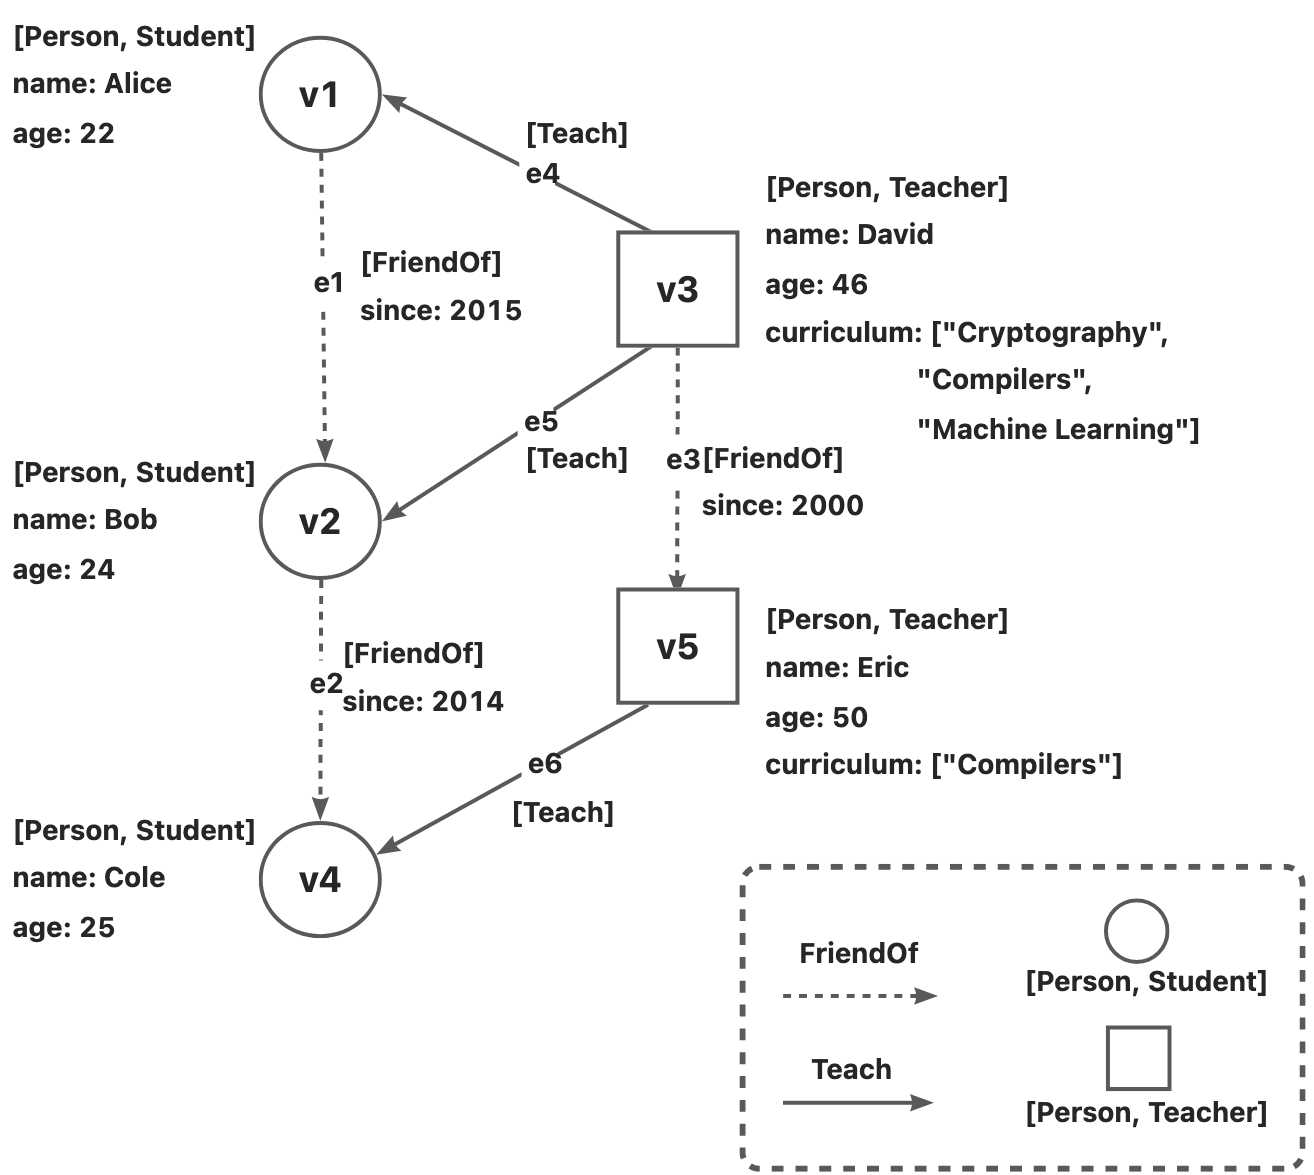
\includegraphics[width=\linewidth]{./figures/example-graph.png}
        \caption{Example Graph.}
        \label{fig:example-graph}
    \end{subfigure}
    \begin{subfigure}[b]{0.4\linewidth}
        \centering
        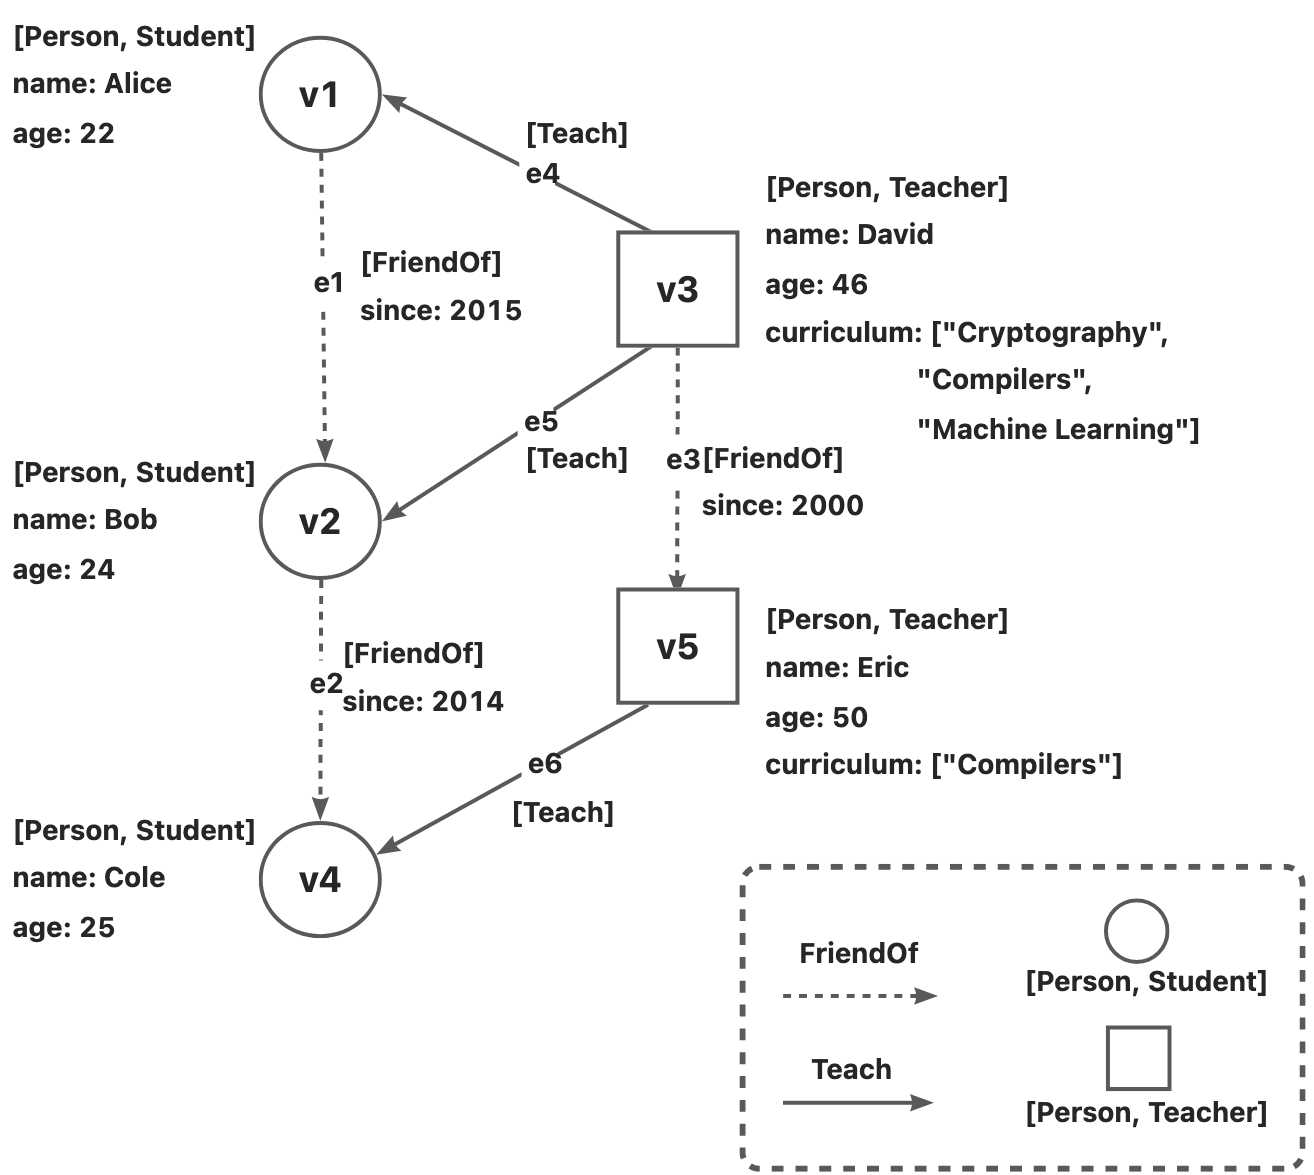
\includegraphics[width=\linewidth]{./figures/example-graph.png}
        \caption{Formal Definition of Example Graph.}
        \label{fig:example-graph-def}
    \end{subfigure}
    \caption{Definition of an example graph.}
    \label{fig:example-graph-full}
\end{figure*}

\begin{example}
    Suppose property graph $G = (V, E, \lambda, L, T, \mathcal{L}, \mathcal{T}, P_v, P_e)$ represents the relationships among persons.
    The property graph is shown in Fig.~\ref{fig:example-graph}.
    Then, to find all the persons with label \text{Student}, the corresponding expression is:
    \begin{equation*}
        \bigcirc_{(v_1\text{:Person})}.
    \end{equation*}
\end{example}


\subsubsection{Selection}

The selection operator is used to filter out the records that do not satisfy the specified constraints.
The formal definition of the selection operator is as follows.

\begin{definition}
    The selection operator is a mapping $\sigma_d : \mathcal{J} \rightarrow \mathcal{J}$, where $d$ represents the constraints the resultant records should satisfy.
\end{definition}

\begin{example}
    To find all the students whose name is ``Bob'', the following expression can be used:
    \begin{equation*}
        \sigma_{v_1.\text{name} = ``Bob''}\bigcirc_{(v_1\text{:Student})}.
    \end{equation*}
\end{example}

\subsubsection{Projection}
The projection operator bridges the gap between graphs and tables, which make it possible to combine graph and relational queries.
Its formal definition is as follows.

\begin{definition}
    The projection operator is a mapping $\pi : \mathcal{J} \rightarrow \mathcal{J}$, which maps vertices and edges to a subset of them or their properties, and maps other attributes to a subset of them.
\end{definition}

Please note that if the resultant records of a projection operator cannot contain any vertex or edge, then it is called a flatten projection operator $\hat{\pi} : \mathcal{J} \rightarrow \mathcal{J}_D$.
A flatten projection operator can convert a property graph to a relational table.

\begin{example}
    Suppose we are going to get a relational table of persons, and the schema of the table is (name, age).
    Then, the following expression can achieve the goal.
    \begin{equation*}
        \pi_{v.name, v.age}(\bigcirc_{(v:Person)}).
    \end{equation*}
\end{example}

\subsubsection{Expand}

The expand operator gets the edges adjacent to the given vertices.
Based on the direction of the expansion, the expand operator can be categorized into three types, i.e., expand-out ($\uparrow$), expand-in ($\downarrow$), and expand-both ($\updownarrow$).
For simplicity, the definition of the expand-both operator is given as follows, and those of expand-out and expand-in are similar.

\begin{definition}
    The expand-both operator is a mapping $\updownarrow_{(v)}^{(w:L)}[e] : \mathcal{J} \rightarrow \mathcal{J}$.
    For each record $c$ containing vertex $v$ and each edge $e$ satisfying $\lambda(e) = (v, w)$ (or $\lambda(e) = (w, v)$), a new record is created by appending ($e$, $w$) to $c$.
\end{definition}
 
\begin{example}
    To get all the ``Teaching''' relationships between students and teachers, the following expression can be used:
    \begin{equation*}
        \downarrow_{(v)}^{(v_t\text{:Teacher})}[\text{:Teaching}]\bigcirc_{(v\text{:Student})}.
    \end{equation*}
\end{example}

\subsubsection{Join}

The join operator can join two relational tables or join two property graphs.
Similar to that in relational algebra, the join operator in graph relational algebra also has many types, such as natural join ($\Join$), left-outer join, and right-outer join.
For simplicity, the definition of natural join is proposed, and those of other types of joins is similar.

\begin{definition}
    The natural join operator $\Join : \mathcal{J} \times \mathcal{J} \rightarrow \mathcal{J}$ combines two relations if they have the same values on common attributes.
\end{definition}

The natural join operator can be expressed as follows:
\begin{equation*}
    \begin{split}
        & R \Join P = \sigma_{R.a_1 = P.a_1 \land \cdots \land R.a_k = P.a_k}(R \times P), \\
        & \hspace{2em} \text{where } \text{attr(sch($R$))} \cap \text{attr(sch($P$))} = \{a_1, \cdots, a_k\}
    \end{split}
\end{equation*}

\begin{example}
    To obtain the names of the teachers who teach the common friends of Alice and Bob, the following expression can be used:
    \begin{equation*}
        \footnotesize
        \begin{split}
            & \pi_{v_3\text{.name}}( \\
            & \hspace{1em} (\downarrow_{(v_c)}^{(v_3\text{:Person})}[\text{:Teaching}]\updownarrow_{(v_1)}^{(v_c\text{:Person})}[\text{:Friend}]\sigma_{v_1\text{.name=``Alice''}}(\bigcirc_{(v_1\text{:Person})})) \\
            & \hspace{1em} \Join (\updownarrow_{(v_2)}^{(v_c\text{:Person})}[\text{:Friend}]\sigma_{v_2\text{.name=``Bob''}}(\bigcirc_{(v_2\text{:Person})}))\\ 
            & )
        \end{split}
    \end{equation*}
\end{example}

\subsubsection{Aggregation}
The aggregation operator groups the records according to the values of the specified attributes, and output new records that may contain aggregated values.
The aggregation operator is denoted by $\gamma_{c_1, \cdots, c_i}^{o_1, \cdots, o_j}$.
Specifically, the records are grouped according to attributes $c_1, \cdots, c_i \in V \cup E \cup D$, and $o_1, \cdots, o_j$ are the outputed new attributes.

\begin{example}
    To count the number of students teached by David, the following expression can be used:
    \begin{equation*}
        \downarrow_{(v_1)}^{(v_s:Student)}[\text{:Teaching}]\sigma_{v_1\text{.name=``David''}}(\bigcirc_{(v_1:Person)})
    \end{equation*}
\end{example}

\subsubsection{Sorting and Top}

The sort operator $\tau_{* a_1, \cdots, * a_n}$ is used to sort the input graph relation according to attributes $a_1, \cdots, a_n \in D$.
Specifically, `*' can be $\uparrow$ or $\downarrow$, representing sorting the records ascendingly or descendingly, respectively.
The results of the sort operator are put in an ordered list rather than a bag.

The top operator $\lambda_k^s$ skips the first $s$ records in the input list, and return the next $k$ records as the outputs.
Since the \emph{bag} semantics are applied in graph relations, the records are unsorted by default and the top operator is meaningless in such bags. 
Therefore, the sort operator is usually applied before the top operator is used.

\begin{example}
    To obtain the most aged five teachers, the utilized expression can be as follows:
    \begin{equation*}
        \lambda_{0}^{5}\tau_{\downarrow \text{age}}(\bigcirc_{(v_1\text{:Teacher})})
    \end{equation*}
\end{example}


\subsubsection{Unwind}

Given a graph relation $R$, suppose attribute $xs \in \text{attr}(\text{sch}(R))$ is a list.
Then, for each record $r$ in $R$, the unwind operator appends each value in $r.x$ to $r$ respectively and removes attribute $xs$ from $r$ to generate new records.
The formal definition of the unwind operator is as follows.

\begin{definition}
    Given graph relation $R$ with $\text{sch}(R) = (a_1, \cdots, a_n)$.
    Without loss of generality, suppose the value of attribute $a_1$ is of list type.
    Then, we have $\text{sch}(\omega_{a_1 \rightarrow a_s}(R)) = (a_2, \cdots, a_n, a_s)$.
    For each record $(val_1, \cdots, val_n) \in R$ with $val_1 = [l_1, \cdots, l_k]$,  $k$ new records are generated, where $r'_j = (val_2, \cdots, val_n, l_j)$, $j \in \{1, \cdots, k\}$.
\end{definition}

\begin{example}
    To get all the classes taught by David, the following expression can be used:
    \begin{equation*}
        \begin{split}
            \pi_{\text{course}}(\omega_{\text{curriculum} \rightarrow \text{course}}(\sigma_{v_1\text{.name=``David''}}(\bigcirc_{(v_1\text{:Person})}))).
        \end{split}
    \end{equation*}
\end{example}


According to SQL/PGQ, the outputs of graph queries should be a relation consisting of property values, identifiers, labels or types.
References to vertices or edges should not be returned by graph queries.
Therefore, the outputs of the graph relational algebra are projected and flattened with the project and unwind operator, respectively.
Then, the output graph relation is converted to a relation over a relational schema, and can be involved in the following optimization of relational optimizer.

\subsection{Equivalence Between Graph Pattern Matching and Graph Relational Operators}

Given a SQL/PGQ query like 
\begin{lstlisting}
    SELECT * 
    FROM GRAPH_TABLE (graph_view
        MATCH <Pattern>
        COLUMNS (
            ...
        )
    );
\end{lstlisting}
the graph query part is expressed with the corresponding graph relational algebra expression with operators such as source, expand, join, and extend-intersect operators, and the logical plan can be generated.
However, the equivalence between the graph relational algebra expression and the graph query is not obvious.
Since the logical plan is finally transformed to a physical plan, which is executed with relational databases, the graph operators for pattern matching such as expand and extend-intersect are indeed implemented with joins.
Therefore, it is necessary to prove that the graph query is the same as its corresponding graph relational algebra expression.

Specifically, <Pattern> specified in the graph query is a list of path patterns, and for each path pattern, a path mode can be given.
In SQL/PGQ, the path mode can be WALK (by default), TRAIL, ACYCLIC, or SIMPLE.
Under the WALK mode, vertices and edges can repeated in the returned results.
Under the TRAIL and ACYCLIC mode, results with repeated edges and vertices are not returned respectively.
Under the SIMPLE mode, results with repeated vertices are not returned, unless these repeated vertices are the first and last vertices in the path (i.e., the path forms a circle).

We start from the case that there is only one path pattern specified in the <Pattern> part, and firstly, we focus on the WALK path mode.
In this mode, paths homomorphic to the path pattern are returned as the results.
Then, we have the following theorem.

\begin{theorem}
    Matching a path pattern in WALK mode have the same meanings as the corresponding graph relational algebra expression. 
\end{theorem}
\begin{proof}
    The graph relational algebra operators related to pattern matching in SQL/PGQ include source, expand, join, and extend-intersect operators.
    Then, we prove the theorem by induction.
    Let each vertex and edge in a path pattern be an element.
    If for each edge in a pattern, its adjacent vertices are also in the pattern, then the pattern is called a strict pattern $P$.
    Otherwise, it is a loose pattern $\hat{P}$.

    Since path patterns specified in SQL/PGQ are all strict patterns, the induction is conducted on the numnber of elements in the strict pattern.
    When there is only one element (i.e., a vertex like ``(u:Label)'') in the pattern, the corresponding algebra expression of the pattern is $\bigcirc_{(u:\text{Label})}$, and it is clear that the expression equals the pattern.

    Then, suppose for a path pattern with at most $n$ elements, the corresponding algebra expressions have the same meaning as matching the path pattern.
    Denote a graph relational algebra with the same meaning as matching path pattern $P$ by $E_p$.
    
    When there are $n + 1$ elements in the path pattern $P$:
    
    %Condition 1: $P = P_1, P_2$, i.e., pattern $P$ is obtained by concatenating subpatterns $P_1$ and $P_2$.
    %(e.g., $P_1 = (u)-[e]-(v), P_2 = (u)-[e']-(w), P = (u)-[e]-(v), (u)-[e']-(w)$).
    %Then, $E_{p_1} \Join E_{p_2}$ equals $P$, since join operator implemented in relational databases follows the semantics of homomorphism.


    Condition 1: $P = P_1 - \hat{P}_2$.
    Without loss of generality, suppose vertex $v$ in $P_1$ is adjacent to an edge in $P_2$.
    (e.g., $P_1 = (u)-[e]-(v), P_2 = [e']-(w), P = (u)-[e]-(v)-[e']-(w)$).
    Then, let $P_3 = (v)-\hat{P}_2$, and the corrsponding algebra expression of $P$ can be $E_{p_1} \Join E_{p_3}$.
    $E_{p_1} \Join E_{p_3}$ equals $P$, since join operator implemented in relational databases follows the semantics of homomorphism.
    Moreover, if $\hat{P}_2$ only consists of one vertex and an edge adjacent to it (i.e., $\hat{P}_2 = [e:eLabel]-(v_t:vLabel)$).
    Then, the corresponding algebra expression of $P$ can also be $\updownarrow_{(v)}^{(v_t:vLabel)}[e:eLabel]E_{p_1}$.
    The expand operator is also implemented by joining relational tables, which follows the semantics of homomorphism.

    Condition 2: $P = P_1$ extends $v$ through edges $e_1:eLabel1, \cdots e_k:eLabelk$ ($k \geq 1$), i.e., at least one vertex in $P_1$ connects to vertex $v$.
    Then, the corresponding algebra expression of $P$ is 
    \begin{equation*}
        E_{p_1} \Diamond_{v_1, \cdots, v_k}^{eLabel1, \cdots, eLabelk} \bigcirc_{(v:vLabel)}.
    \end{equation*}
    Since the extend-intersect operator is implemented with relational joins and follows the semantics of homomorphism, the algebra expression has the same meaning as matching the path pattern.

    In conclusion, the corresponding algebra expressions of path pattern $P$ with $n + 1$ elements have the same meaning as matching the path pattern.

    In conclusion, in the WALK mode, matching path patterns has the same meaning as the corresponding graph relational algebra expressions.
\end{proof}


Besides the WALK mode by default, when the path patterns are in TRAIL, ACYCLIC, or SIMPLE mode, we still have the same conclusions.
Specifically, in TRAIL, ACYCLIC, or SIMPLE mode, a selection operator needs to be added to remove the results with repeated edges or vertices.
In detail, the selection operator should wrap the corresponding algebra expression of path patterns in the WALK mode.
For example, in the TRAIL mode, the corresponding graph relational algebra expression of $P = P_1 - P_2$ is $\sigma_{c}(E_{p_1} \Join E_{p_2})$ or $\sigma_{c}(\updownarrow_{(v)}^{(v_t:vLabel)}[e:eLabel]E_{p_1})$, where $c$ is the condition specifying that every two different pattern edges bind to different edges in each result.
In the ACYCLIC and SIMPLE mode, condition $c$ should be specified according to the constraints of the mode.

Furthermore, there may be more than one path patterns specified in the <Pattern> part of SQL/PGQ queries, and the different path patterns may have different path modes.
Denote the path patterns by $P_1, \cdots, P_k$.
According to SQL/PGQ, the binding results of different path patterns are joined together.
If the match mode in SQL/PGQ is set to \textbf{REPEATABLE ELEMENTS}, there is no more constraint, and ``MATCH $P_1, \cdots, P_k$'' has the same meaning as $P_1 \Join \cdots \Join P_k$, both of which have the semantics of homomorphism.
Otherwise, if the match mode in SQL/PGQ is set to \textbf{DIFFERENT EDGES}, the same edge cannot bind to different variables in different path patterns.
Therefore, a selection operator is needed, and ``MATCH $P_1, \cdots, P_k$'' has the same meaning as $\sigma_{d}(P_1 \Join \cdot \Join P_k)$, where $d$ is the condition specifying that each edge cannot bind to more than one variables across all path patterns.

\section{Converged Graph Relational Optimization Framework}

In this section, we first introduce the sketch of the converged graph relational optimizer.
Then, Section \ref{sec:framework:combination} presents the workflow of the framework, and Section \ref{sec:framework:detailed-optimizations} explains the optimization strategies applied in the framework in detail.

\begin{figure}
    \centering
    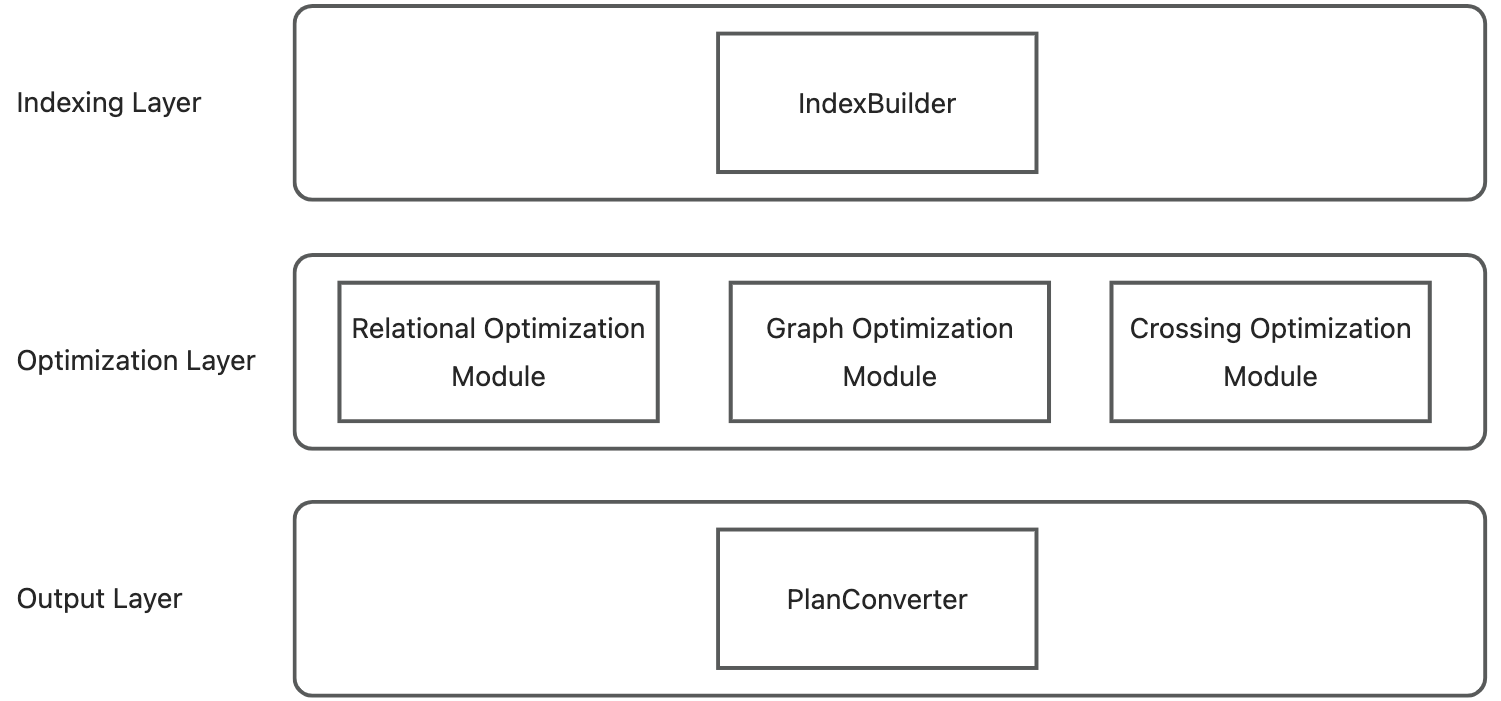
\includegraphics[width=\linewidth]{./figures/framework.png}
    \caption{Overview of the Converged Graph Relational Optimization Framwork.}
    \label{fig:framework-overview}
\end{figure}

\subsection{Overview of the Framework}

% A system overview figure and some introduction
The framework consists of three layers as shown in Fig.~\ref{fig:framework-overview}, i.e., indexing layer, optimization layer, and output layer.
In this subsection, the details of these three layers are introduced in detail.

\textbf{Indexing Layer.} The indexing layer mainly builds graph indices for the graph optimization module with IndexBuilder.
For the graph queries specified in the SQL/PGQ query, the obtained graph plans are likely to contain the commonly used graph operators (e.g., \textit{GetVertex}, \textit{GetEdge}, and \textit{GetNeighbor}).
However, traditional relational databases cannot support such operators efficiently.
Therefore, graph indices need to be constructed so that vertices can efficiently access its adjacent edges and neighboring vertices, and edges can also quickly obtain their adjacent vertices.
Then, in the process of optimizing the graph subplans, the cost of graph operators like \textit{GetNeighbor} should be that of obtaining neighbors of vertices in relational databases with graph indices.

\textbf{Optimization Layer.} The optimization layer consists of three modules, i.e., the relational optimization module, graph optimization module, and crossing optimization module.
In detail, the relational optimization module optimizes relational queries with relational optimization strategies.
It should contain rule-based optimizations (abbr.~RBOs) and cost-based optimizations (abbr.~CBOs), and can be any one of the commonly used relational optimizers (e.g., Calcite or the optimizer of Duckdb).
The graph optimization module optimizes graph queries and also has specific RBOs and CBOs for graphs queries.
It can be any existing graph optimizer (e.g., GLogue).
Besides, the crossing optimization module optimizes the relational queries and graph queries simultaneously.
Optimizations are achieved through interaction and transformation between relational and graph queries.

\textbf{Output Layer.} The output layer converts the execution plan obtained in the optimization layer to the plan that can be executed by the target database.
To ensure the flexibility of the framework, codegen technology is utilized to implement the PlanConverter.
In detail, the PlanConverter first converts the obtained execution plan into the predefined internal representation, and then the internal representation is transformed into a physical plan that the target database can parse and execute.

\begin{figure}
    \centering
    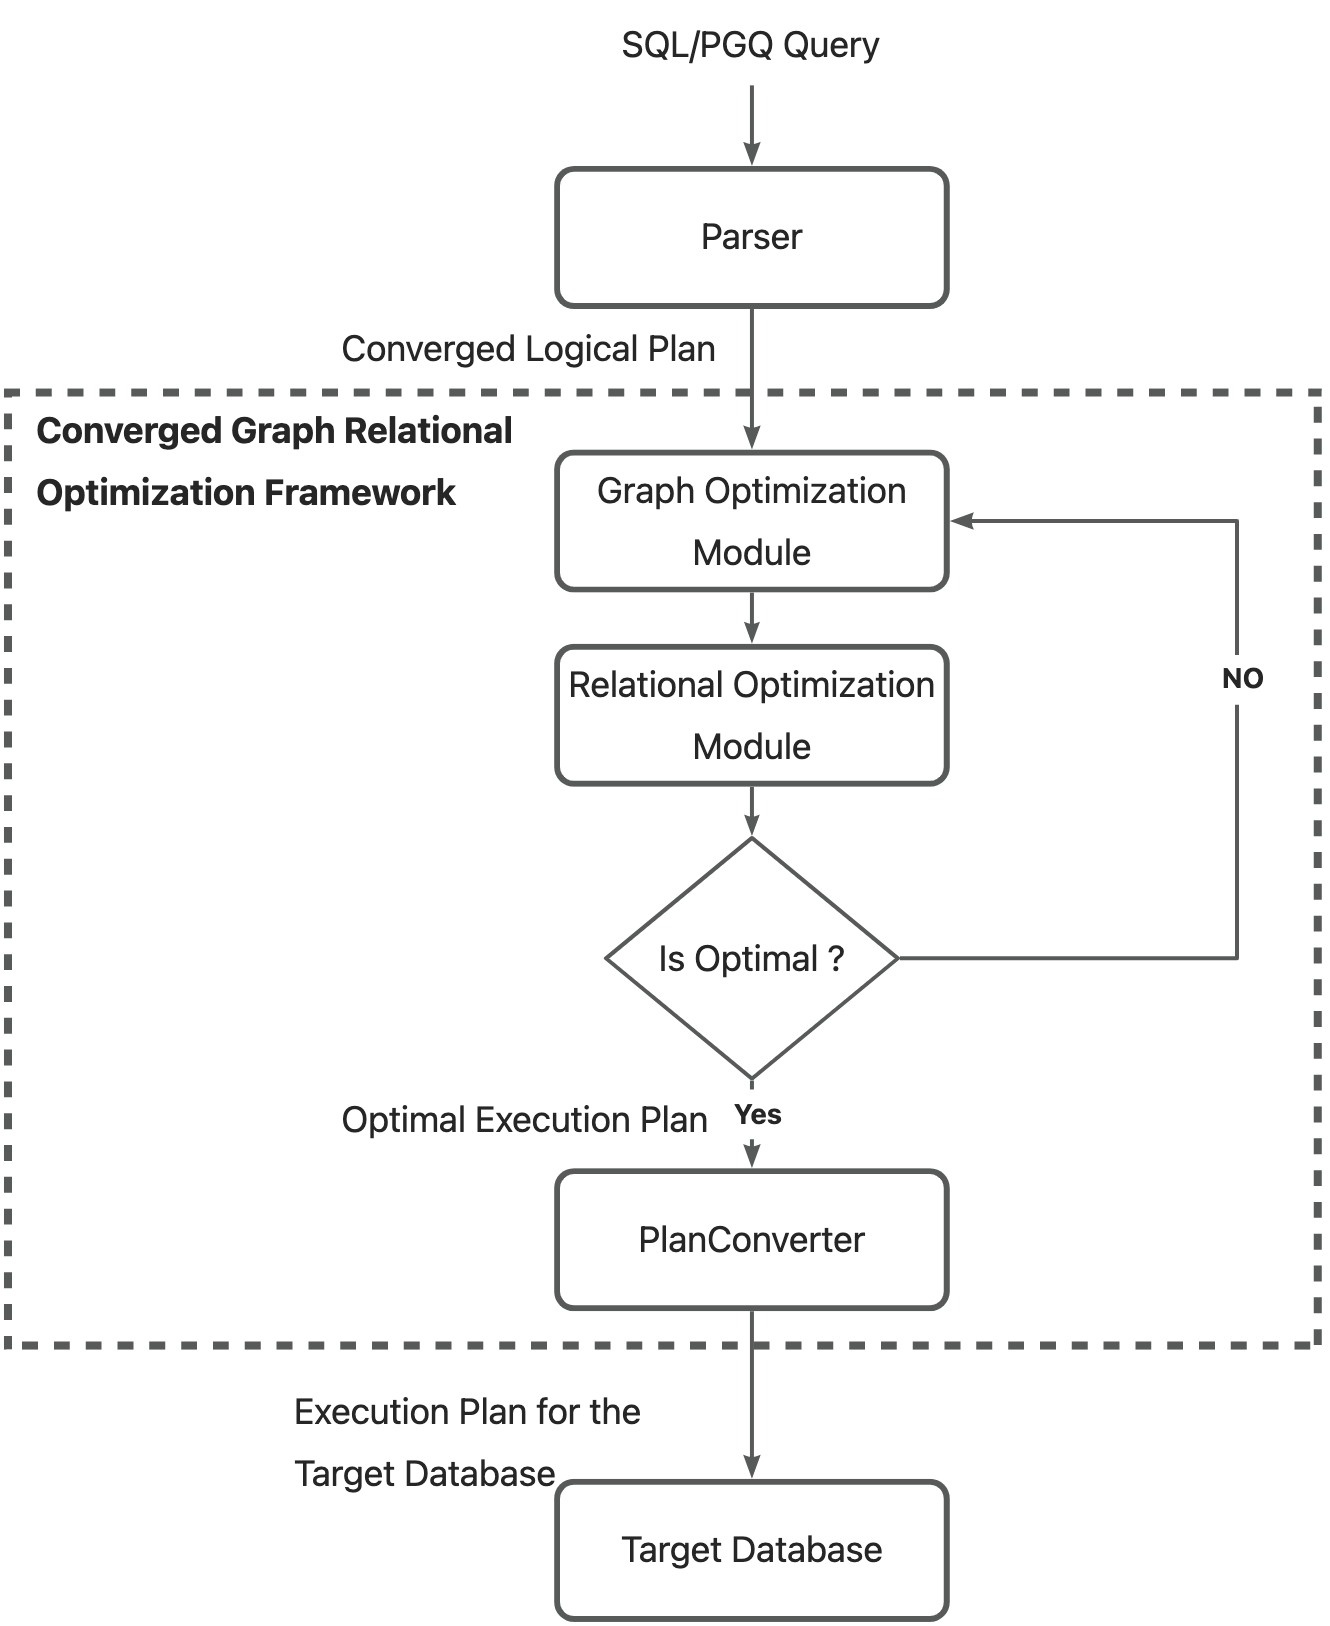
\includegraphics[width=\linewidth]{./figures/workflow.png}
    \caption{Workflow of the Converged Graph Relational Optimization Framework.}
    \label{fig:workflow}
\end{figure}

\subsection{Leveraging Benefits of Both Relational and Graph Optimizations}
\label{sec:framework:combination}

\begin{figure*}
    \centering
    \begin{subfigure}[b]{0.4\linewidth}
        \centering
        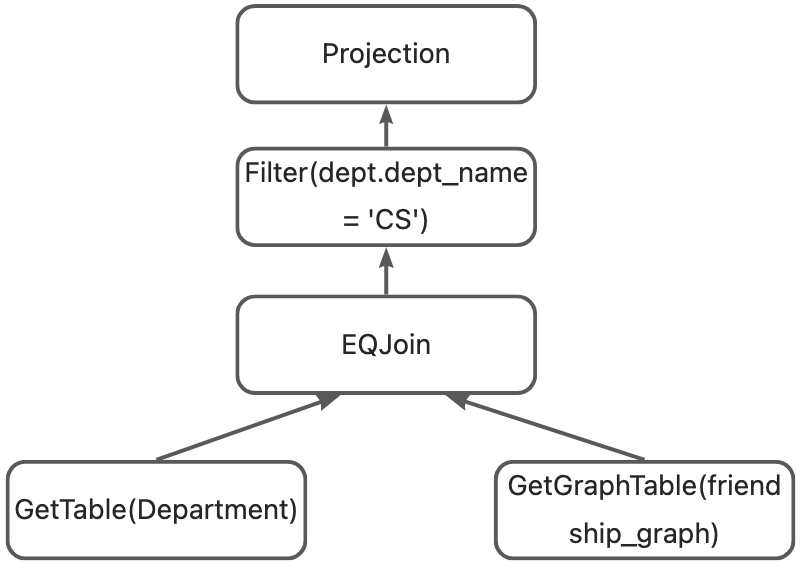
\includegraphics[width=\linewidth]{./figures/converged-logical-plan-relational.png}
        \caption{Relational Subplan of the Converged Logical Plan.}
        \label{fig:converged-logical-plan-relational}
    \end{subfigure}
    \begin{subfigure}[b]{0.4\linewidth}
        \centering
        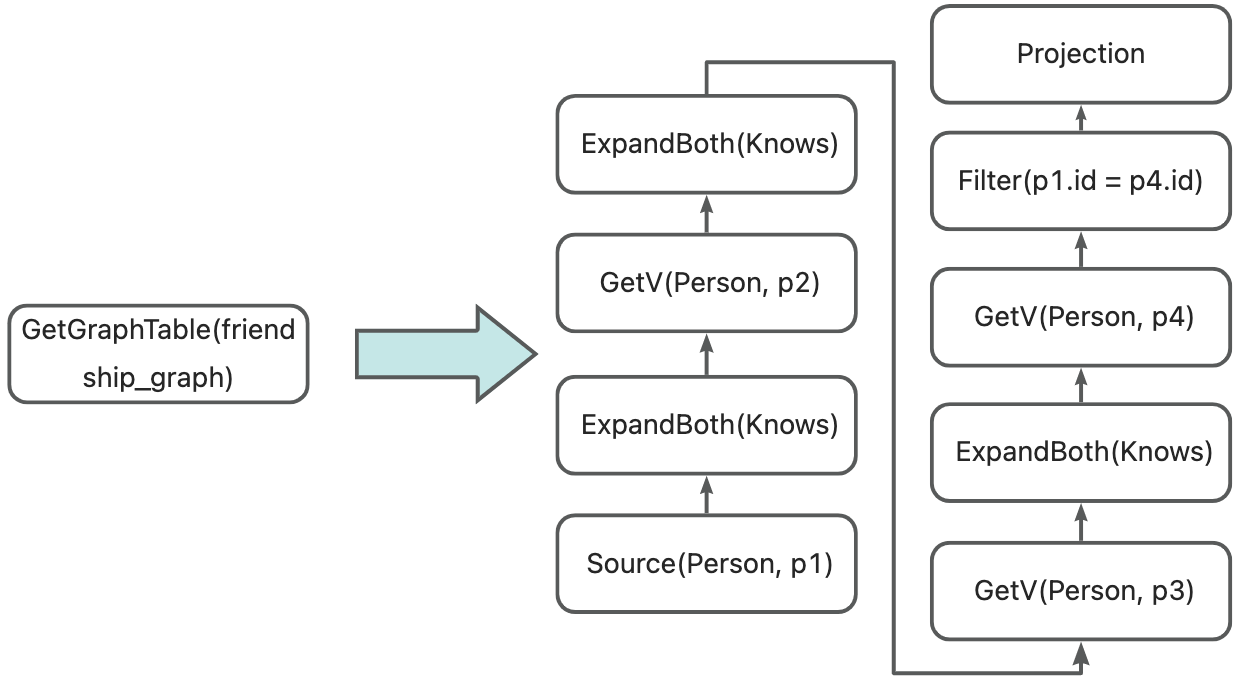
\includegraphics[width=\linewidth]{./figures/converged-logical-plan-graph.png}
        \caption{Graph Subplan of the Converged Logical Plan.}
        \label{fig:converged-logical-plan-graph}
    \end{subfigure}
    \begin{subfigure}[b]{0.4\linewidth}
        \centering
        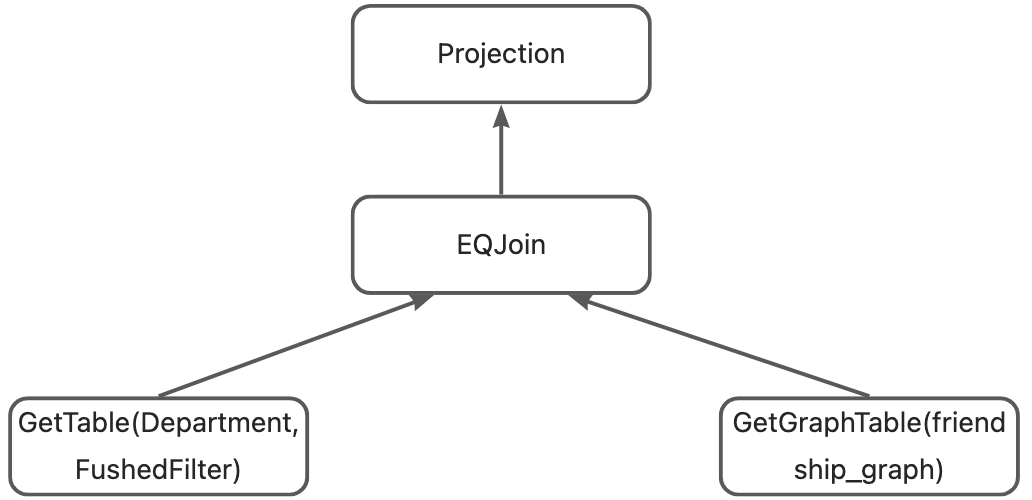
\includegraphics[width=\linewidth]{./figures/converged-logical-plan-relational-optimized.png}
        \caption{Relational Subplan after Optimization.}
        \label{fig:relational-plan-optimized}
    \end{subfigure}
    \begin{subfigure}[b]{0.4\linewidth}
        \centering
        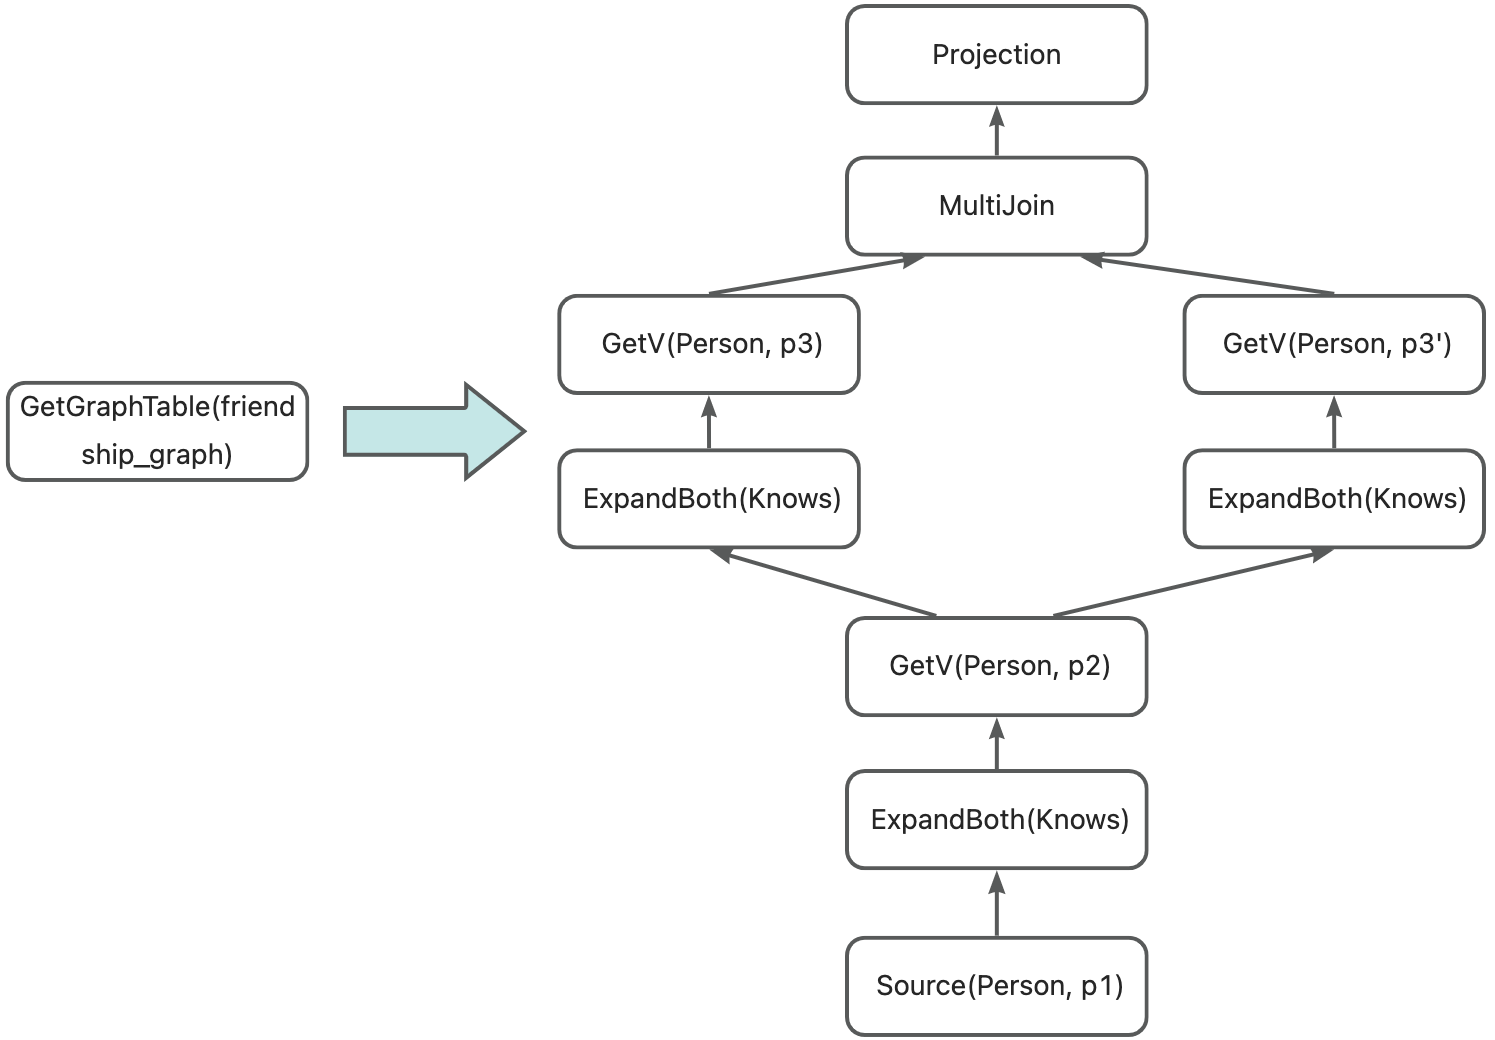
\includegraphics[width=\linewidth]{./figures/converged-logical-plan-graph-optimized.png}
        \caption{Graph Subplan after Optimization.}
        \label{fig:graph-plan-optimized}
    \end{subfigure}
    \begin{subfigure}[b]{0.4\linewidth}
        \centering
        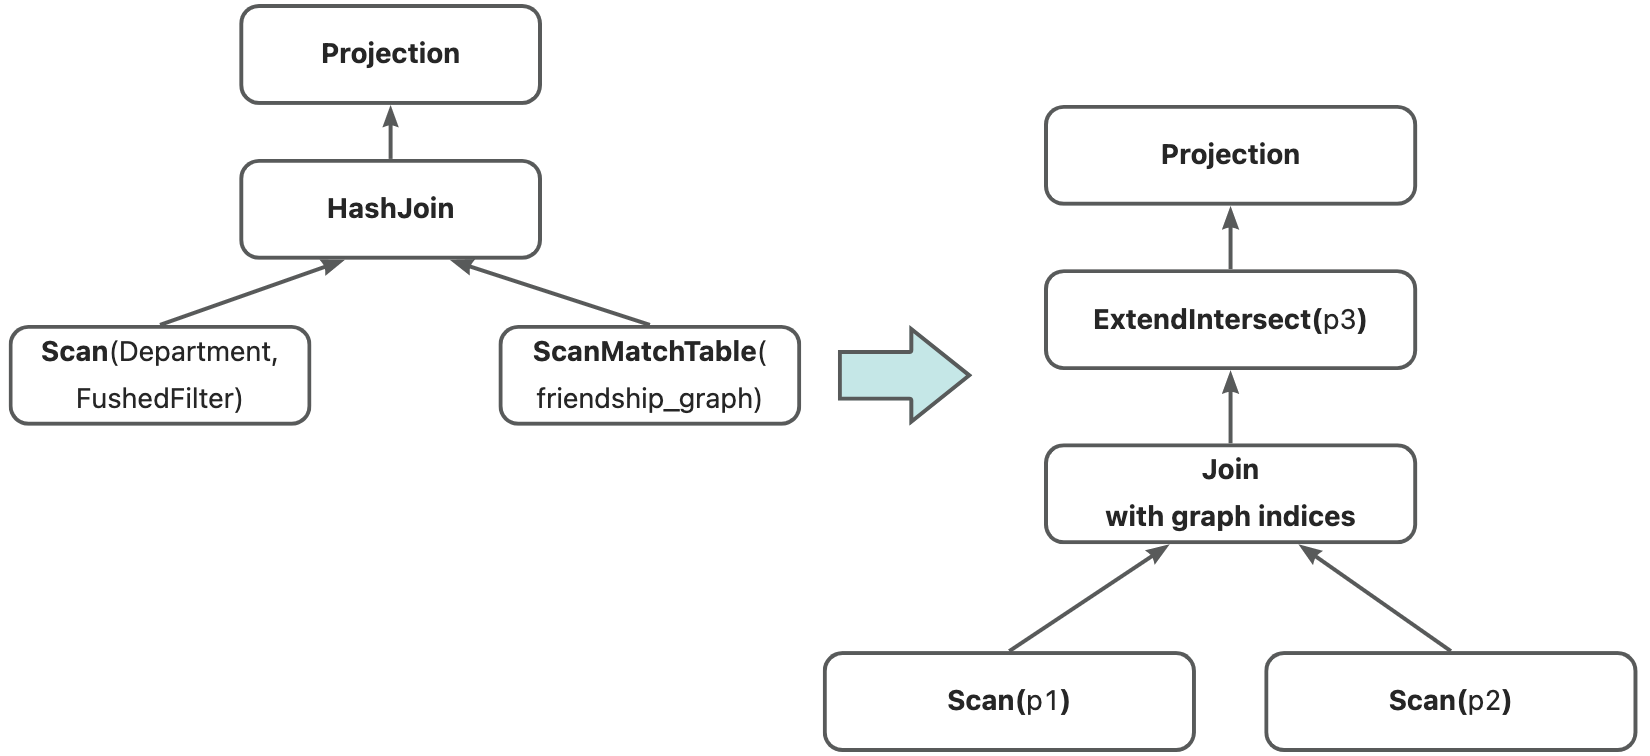
\includegraphics[width=\linewidth]{./figures/converged-physical-plan.png}
        \caption{Obtained Optimial Physical Plan.}
        \label{fig:physical-plan-optimized}
    \end{subfigure}
    \caption{An example of query opitmization.}
    \label{fig:query-grtree-example}
\end{figure*}


Fig.~\ref{fig:workflow} illustrates the workflow for optimizing a query that adheres to the SQL/PGQ grammar using the converged graph relational optimization framework.
In detail, the query is first parsed and a converged logical plan is generated.
The converged logical plan consists of several graph subplans and a relational subplan.
Eacn graph subplan corresponds to a graph query, and it is optimized with the graph optimization module.
Since parts of the graph query are always marked with ``GRAPH\_TABLE (name, MATCH $\cdots$)'', it is straightforward to distinguish graph queries from relational queries, and the graph subplans can be generated easily.
For each graph subplan, an operator ``GetGraphTable(name)'' is generated and added to the relational subplan.
Specifically, from the perspective of the relational optimization module, the ``GetGraphTable'' operator is simply an operator for retrieving data like ``GetTable'' and it returns table data.
Please note that since the outputs of graph queries need to be relational tables as defined in SQL/PGQ, a graph query can be utilized as a subquery to retrieve the table involved in the relational query.
However, a relational query cannot serve as a subquery within a graph query because the mappings between relational tables and vertices/edges need to be specified beforehand, and the graph indices should be built in advance.


With the generated converged logical plan, the converged optimizer takes effect and obtains the optimal physical plan with the modules in the optimization layer.
Specifically, the crossing optimization module first takes effects, e.g., pushing filtering conditions from the relational subquery to graph subqueries.
Then, the graph subqueries are optimized with the graph optimization module.
During the process of optimizing the graph subqueries, the cardinalities of the outputs of the graph subqueries are also estimated.
Next, the relational optimization module is utilized to optimize the relational query, where some source tables may be the outputs of graph subqueries.
After that, it is tested whether the crossing optimization module can further optimize the plan.
If the plan can still be optimized, then the three modules are applied again to optimize the plan.
Otherwise, the optimal execution plan is obtained.

After the optimal physical plan is obtained, the PlanConverter transforms the plan to an internal representation (e.g., substrait), and then the internal representation is transformed to the physical plan that can be executed by the target database.
Finally, the plan is executed and the query results are obtained.
The above process of query processing is illustrated with the following example.

\begin{example}
    Given a relational database with tables as follows,
    \begin{equation*}
        \begin{split}
            & \textit{Person = (\underline{id}, name, dept\_id)} \\
            & \textit{Knows = (\underline{id1}, \underline{id2})} \\
            & \textit{Department = (\underline{dept\_id}, dept\_name)}, \\
        \end{split}
    \end{equation*}
    suppose we are going to find three persons satisfying: 
    (1) These three persons know each other;
    (2) At least two of them are from the department of computer science.
    The SQL/PGQ query for this task is shown in Example \ref{example:introduction:sqlpgq}.      

    There is one graph query for obtaining triangles of persons that know each other.
    Therefore, the converged logical plan consists of one relational subplan and one graph subplan.
    The algebra expression corresponding to this query is as follows:
    Firstly, to obtain the triangles, the graph relational algebra expression is
    \begin{equation*}
        \begin{split}
            G_{\triangle} = & \sigma_{p4.id = p1.id}(\updownarrow_{(p3)}^{(p4)}[:Knows]\updownarrow_{(p2)}^{(p3:Person)}[:Knows] \\
            & \updownarrow_{(p1)}^{(p2:Person)}[:Knows]\bigcirc_{(p1:Person)}).
        \end{split}
    \end{equation*}
    Then, to get the results of the graph query and formulate the results as a relational table, the algebra expression is 
    \begin{equation*}
        \begin{split}
            R_{graph} = & \pi_{p1.name\rightarrow pn1, p1.dept\_id \rightarrow dept1,p2.name\rightarrow pn2, p2.dept\_id \rightarrow dept2,} \\
            & _{p3.name\rightarrow pn3, p3.dept\_id \rightarrow dept3}(G_{\triangle}).
        \end{split}
    \end{equation*}
    Finally, to obtain the triangles of persons with at least two persons from the department of computer science, the relational algebra expression is
    \begin{equation*}
        \begin{split}
        \pi_{pn1, pn2, pn3}
        (& \sigma_{dept.dept\_name = `Computer Science'}( \\ 
        & dept \Join_{dept1=dept.dept\_id \land dept2=dept.dept\_id} R_{graph})).
        \end{split}
    \end{equation*}

    Based on the above algebra expressions, the corresponding converged logical plan is shown, and its relational and graph subplans are presented in Fig.~\ref{fig:converged-logical-plan-relational} and Fig.~\ref{fig:converged-logical-plan-graph}, repsectively.
    
    Then, optimization modules in the optimization layer are applied to optimize the relational subplan and graph subplans.
    The optimized converged logical plan is shown in Fig.~\ref{fig:relational-plan-optimized} and Fig.~\ref{fig:graph-plan-optimized}.
    Moreover, the finally obtained optimal physical plan is shown in Fig.~\ref{fig:physical-plan-optimized}.
\end{example}

\subsection{Detailed Optimizations}
\label{sec:framework:detailed-optimizations}

In this subsection, we first present the optimization strategies utilized in the relational optimization module and graph optimization module, respectively.
Then, the strategies of crossing optimization module are also proposed.

\subsubsection{Optimization Strategies in Relational Optimization Module}

Like most relational optimizers, the relational optimization module applies both Rule-based Optimization (abbr.~RBO) and Cost-based Optimization (abbr.~CBO) strategies on relational subplans for a better physical plan.
In detail, in terms of RBO, commonly used optimizations such as filter pushdown, join order optimization, and removal of unused columns are employed in the converged optimizer.
In terms of CBO, the costs of plans are estimated based on the low-order statistics such as the cardinalities of tables and query conditions.



\subsubsection{Optimization Strategies in Graph Optimization Module}

In the graph optimization module, we formulate a specific rule set to capitalize on optimization potential among graph operators. 
Both RBO and CBO strategies are included in the rule set.

In terms of RBO strategies, two frequently utilized key rules, i.e., \trimrule and \fusionrule, are presented in this subsection.

\trimrule. 
The \trimrule~ is a well-established relational optimization strategy that removes superfluous data at intermediary stages of query processing. 
Two particular instances where trimming helps include: 
Firstly, \trimrule~ can eliminate intermediate results with aliases that are not required and reduce computations.
Secondly, it involves discarding unneeded vertex and edge properties when retrieving from the data graph. 
This is accomplished by specifying essential properties in the graph operators’ \code{COLUMNS} field.
Formally, an example of applying \trimrule is as follows:
\begin{equation}
    \mathcal{S}_g \Rightarrow \pi_{u.a_1, \cdots, u.a_k}\mathcal{S} _g 
\end{equation}
where $\mathcal{P}_g$ is a graph relational algebra expression corresponding to a graph subplan, and $u.a_1, \cdots, u.a_k$ are necessary properties.


\fusionrule. 
The \fusionrule~ is a graph-centric rule. 
Commonly in graph queries, a sequence of \expandedge~ followed by \getvertex~ indicates a search for neighboring vertices. 
The \fusionrule~ consolidates these operators into one integrated \expandvertex~ to boost efficiency. 
Nonetheless, whether \expandedge~ and \getvertex~ can be merged is context-dependent. 
For example, if some properties of the edges are needed, fusion might not be feasible.
This rule evaluates such factors to ensure query optimization without compromising result integrity.
%Formally, an example of applying \fusionrule is as follows:
%\begin{equation}
%    \begin{split}
%    &  \\
%    & \hspace*{2em} \Rightarrow \pi_{u.a_1, \cdots, u.a_k}\updownarrow_{(u)}^{(v:vLabel)}[:eLabel](\sigma_{d(u)}\bigcirc_{(u:uLabel)}), \\
%    \end{split}
%\end{equation}
%where $d(u)$ is a filtering constraint on vertex $u$.


In terms of CBO, drawing from insignts gained in the prior research, we implement effective pattern matching by incorporating hybrid pattern join strategies and leveraging high-order statistics, which provide a more granular understanding of the data through the frequency of smaller patterns.
Moreover, the prior research has some drawbacks, including using a bottom-up search framework that potentially missed early pruning opportunities and having a narrow focus on basic patterns without accommodating union patterns scenarios.
Therefore, we also introduce a novel top-down search framework, inclusive of branch-and-bound pruning strategies, and devise specific cardinality estimation methods for union patterns. 
Besides, in this implementation, we use a rule for pattern transformation to ensure all modifications maintain the original results’ integrity.
Furthermore, for pattern matching, we consider binary join and extend-intersect operators. 
The binary join applies a hash-join on two pattern mappings to produce a larger pattern's results.
The extend-intersect operator optimizes the process when only one vertex is added to the existing pattern. 
This expansion can vary from a simple addition of a single new edge to more complex scenarios involving multiple edges, implemented through optimal joins.

Regarding cost and cardinality estimation, we adopt a cost model that considers both the communication costs of intermediate result transfer in distributed environments and the computational costs of physical plan operators. 
Specifically, costs for the binary join and extend-intersect operators in graphs are defined. 
Additionally, we estimate the operator cost using an expand ratio that reflects the change in pattern occurrences when edges are expanded.

\subsubsection{Optimization Strategies in Crossing Optimization Module}

Please note that the optimizations of graph subplans and the relational subplan are not isolated or entirely unconnected.
For example, when \trimrule~ is applied on graph subplans, it is necessary to judge whether the properties of vertices and edges are utilized in graph subplans and relational subplans.
Actually, more crossing optimization strategies can be designed for optimizing the graph and relational subplans simultaneously.
Such optimizations are included in the crossing optimization module, and two typical and crucial strategies of them are \filterrule and \intersectrule. 

\filterrule. 
The \filterrule seeks to push filtering conditions on properties of graph elements from the relational subplan to graph subplans, so that invalid graph elements can be dropped earlier.
An example of applying \filterrule is given in Example \ref{example:push_down}.

Specifically, \filterrule can embed filtering conditions into basic graph operators like \scan~, \expandedge~, or \getvertex~ to further push down filtering conditions in graph queries. 
This integration allows the direct exclusion of vertices and edges not satisfying the filter conditions, thus drastically cutting down the volume of intermediary outcomes.

Formally, the equation rule w.r.t.~\filterrule is as follows:
\begin{equation}
    \begin{split}
    & \sigma_{\theta}\pi_{v.a_1, \cdots, v.a_k}(lr~\alpha_{(u)}^{(v)}[e]~er) \\
    & \hspace*{2em} \equiv \pi_{v.a_1, \cdots, v.a_k}(lr~\sigma_{\theta}(\alpha_{(u)}^{(v:vLabel)}[e]~er)), \\
    \end{split}
\end{equation}
where $lr$ and $er$ are graph relational algebra expressions, $\alpha \in \{\uparrow, \downarrow, \updownarrow\}$, and vLabel is specified if the label of $v$ is specified in $\theta$.


\intersectrule. 
Please note that the intersection operator is not defined in graph queries, but it can be expressed with expand operators.
Given a SQL/PGQ query, if the two subqueries that intersect are both graph queries, then the paths in these two graph queries can be combined with expand operators to generate new paths.
That is, two graph queries combined with an intersection operator is converted to a new graph query.
By leveraging graph indices, it can be more efficient to obtain the intersection results w.r.t.~the new graph query.
The rule is as follows.
\begin{equation}
    \begin{split}
        & \pi_{u.a_1, \cdots, u.a_k}(el~\alpha_{(u)}^{v:vlabel}[e]~er) \\
        & \hspace*{2em} \equiv \pi_{u.a_1, \cdots, u.a_k}(el) \cap \pi_{u.a_1, \cdots, u.a_k}(\alpha_{(u)}^{v:vlabel}[e]~er),
    \end{split}
\end{equation}
where $el$ and $er$ are graph relational algebra expressions, $\alpha \in \{\uparrow, \downarrow, \updownarrow\}$.
\section{Superiority of the Graph Optimizer on Graph Queries}
\label{sec:theoretical-analysis}

In this section, we prove that graph optimizers have better performance than relational optimizers.
Besides, since graph optimizers cannot always be used to optimize relational queries, it confirms the necessity of proposing the converged query optimization.

As one of the most widely adopted optimizers for relational databases, we use Calcite \cite{calcite,columbia} as a representative of relational JOPTs and analyze its efficiency of join order optimization.
For the converged JOPT, we use GLogue \cite{GLogS} as the graph JOPT, and integrate it with Calcite.

A more simple condition is first considered.
That is, all the tables in the query can represent vertices or edges.
Then, it is supposed that there are $n + m$ tables are joined together, where $n$ tables represent vertices while $m$ tables represent edges.
Suppose that there are $t$ implementation methods for join.
The complexities of optimizing the join order with Calcite and the converged JOPT are analyzed respectively as follows.
For simplicity, the time complexities are evaluated by the number of physical plans generated by the JOPTs.

\begin{theorem}
    \label{theorem:complexity-of-calcite}
    The time complexity of join order optimization with Calcite is at least $O(\frac{4^{m+n-1}}{m+n}t^{m+n-1})$.
\end{theorem}
\begin{proof}
    The $n + m$ tables joined together can form a graph, where the tables represent vertices in the graph, and if there is a join condition specifying the equivalence of two columns in two two tables, there is an edge between these two tables.
    Then, the complexity of join order optimization with Calcite can be estimated as the number of possible physical plans that can be generated.
    
    To avoid cross product, except for the first table, the selected tables to be be joined with the already chosen tables should be neighbors of the chosen tables in the graph.
    Therefore, the join order can be represented as a spanning tree in the graph.
    By computing the number of physical plans can be generated according to each spanning tree, the total number of physical plans can be obtained.
    However, same phyical plans may be obtained according to different spanning trees.
    For example, suppose a graph is a rectangle with four vertices and four edges.
    It may be constructed for a query like:
    \begin{equation*}
        \begin{split}
            \text{SELECT}\hspace{.5em} ... & \hspace{.5em}\text{FROM}\hspace{.5em} A, B, C, D \hspace{.5em}\text{WHERE}\hspace{.5em} A.1 = B.1 \\ 
            & \hspace{.5em}\text{AND}\hspace{.5em} B.2 = C.1 \hspace{.5em}\text{AND}\hspace{.5em} C.2 = D.1 \hspace{.5em}\text{AND}\hspace{.5em} D.2 = A.2. 
        \end{split}
    \end{equation*}
    Then, the spanning tree with edges \{AB, BC, CD\} and the one with edges \{AB, BC, AD\} can generate same physical plans.
    Consequently, the summation of the number of physical plans corresponding to all the spanning trees is larger than the actual number of physical plans.
    In this proof, we compute the number of physical plans for one spanning tree, and this number is the lower bound of the number of physical plans that can be generated.

    Given a spanning tree with $k$ edges (i.e., $k+1$ vertices representing tables) and only one leaf node, the number of logical plans corresponding to the spanning tree is roughly
    \begin{equation*}
        \begin{split}
            c(k) & = 2 * (c(0)c(k-1) + c(1)c(k-2) + \cdots + c(k-1)c(0)) \\
            & = 2\Sigma_{i=0}^{i=k-1}c(i)c(k-1-i), \\
            & \text{where } c(0) = 1.
        \end{split}
    \end{equation*}
    With the generating function, it is obtained that 
    \begin{equation*}
        c(k) = \frac{2^k}{k+1}C(2k, k).
    \end{equation*}
    Since $k$ is the number of edges, and $k = m + n - 1$ in the spanning tree.
    Thus, the number of logical plans w.r.t.~a spanning tree is 
    \begin{equation*}
        \frac{2^{m+n-1}}{m+n}C(2m+2n-2, m+n-1) \geq \frac{4^{m+n-1}}{m+n}.
    \end{equation*}
   Then, the number of physical plans is at least $\frac{4^{m+n-1}}{m+n}t^{m+n-1}$, so is the complexity of join order optimization with Calcite.
   
   In conclusion, Theorem \ref{theorem:complexity-of-calcite} is correct.
\end{proof}

\begin{lemma}
    \label{lemma:upper-bound-of-calcite}
    Given $n$ tables, the time complexity of join order optimization with Calcite has an upper bound of $O(\frac{(2n-2)!}{(n-1)!}t^{n-1})$.
\end{lemma}
\begin{proof}
    The upper bound of the time complexity of join order optimization is achieved when there is a condition between any two of the $n$ tables.
    Because at that time, the tables can be joined in any order.

    Since each join order corresponds to a full binary tree with $2n-1$ nodes, the problem is to count the number of possible full binary trees.
    Similar to Catalan number, the number of full binary trees is $O(C(2n-2, n-1) - C(2n-2, n))$.
    For each full binary tree, there are $n!$ ways to set the leaf nodes. 
    Then, the number of generated physical plans is $O(\frac{(2n-2)!}{(n-1)!}t^{n-1})$.
\end{proof}

\begin{theorem}
    \label{theorem:complexity-of-glogue}
    The time complexity of join order optimization with the converged JOPT is smaller than $3^n$ if all the tables participant in join can represent vertices or edges.
\end{theorem}
\begin{proof}
    Since the $n + m$ tables represent vertices and edges respectively and the join among them can be represented as a graph query, the converged JOPT optimizes the join order with the graph optimizer, i.e., GLogue.

    As GLogue ensures worst-case optimality and the considered patterns are all induced subgraphs, the time complexity of join order optimization with GLogue is not related to the number of edges (i.e., $m$).
    Because JOOP is reduced to a variant of shortest path problem, the time complexity of join order optimization is $O(\mathcal{E})$, where $\mathcal{E}$ is the number of edges in GLogue.
    In detail, 
    \begin{equation*}
        \begin{split}
            O(\mathcal{E}) & = C(n, n-1)*(2^{n-1}-1) + C(n, n-2) * (2^{n-2}- 1) \\
            & + \cdots + C(n, 1) * (2^1 - 1) \\
            & = 3^n - 2^{n+1} +1 \\
            & < 3^n.
        \end{split}
    \end{equation*}
    
    In conclusion, Theorem \ref{theorem:complexity-of-glogue} is correct.

\end{proof}

Based on the complexity analysis in Theorem \ref{theorem:complexity-of-calcite} and Theorem \ref{theorem:complexity-of-glogue}, it is found that when the tables represent vertices and edges, 
\begin{equation*}
    \begin{split}
        \frac{\text{Time Complexity of Calcite}}{\text{Time Complexity of the Converged JOPT}} & = \frac{\frac{4^{m+n-1}}{m+n}}{3^n}t^{m+n-1} \\
        & \geq 2^{m-3}(\frac{4}{3})^nt^{m+n-1}.
    \end{split}
\end{equation*}
Therefore, it suggests that the converged JOPT is exponentially faster than Calcite for graph-like join order optimization.
The results also indicates that integrating graph optimizers into relational optimizers can improve the efficiency of join order optimization significantly.


Then, if there are some tables that cannot represent vertices or edges, the order of such tables cannot be optimized with graph optimizers, and the comparion becomes more complicate.
For example, suppose five tables form a clique, and then these tables cannot be vertices or edges in a graph.
Specifically, according to the dataflow shown in Fig.~\ref{fig:dataflow}, the join order of these left tables are optimzed by relational optimizers such as Calcite.
Let the number of left tables be $s$, and together with the table obtained by the join of the tables optimized with graph optimizer, Calcite needs to optimize the join order among $s + 1$ tables.

When $s = 0$, all the tables represent vertices or edges, and the time complexity of the converged JOPT is exponentially smaller than that of Calcite as analyzed as above.

When $s = 1$, only one table (saying $T_1$) does not represent a vertex or an edge, and Calcite optimizes the join between two tables.
One of these two tables is $T_1$, and the other is the table obtained by the join of the tables optimized with graph optimizer.
Then, we have
\begin{equation*}
    \begin{split}
        \frac{\text{Time Complexity of Calcite}}{\text{Time Complexity of the Converged JOPT}} > \hspace{-12em} & \\
        & \frac{\frac{2^{m+n-1}}{m+n}C(2m+2n-2, m+n-1)t^{m + n - 1}}{3^{\hat{n}} + \frac{(2s)!}{(s)!}t^{s}} \\
        & = \frac{\frac{2^{m+n-1}}{m+n}C(2m+2n-2, m+n-1)t^{m + n - 1}}{3^{\hat{n}} + 2} >> 1,
    \end{split}
\end{equation*}
where $\hat{n}$ is the number of tables representing vertices.
It indicates the superiority of the converged JOPT.

When $s = m + n - 1$ or $p = m + n$, at most one table can represent vertices or edges, and the converged JOPT degenerates to Calcite, and has the same efficiency as it.
A typical example is when there is a condition between any two of these $m + n$ tables.

The results show that the converged JOPT is always superior to relational JOPTs.
To be more specific, we prove the superiority of the converged JOPT more theoretically.

\begin{lemma}
    \label{lemma:join-spliter}
    Let $\text{JN}_c(V_s)$ represent the number of possible physical plans of joining tables in table set $V_s$ with Calcite.
    Suppose $n$ tables (denoted as table set $V$) are joined, and $V = (V_1 - u) \cup V_2$, $V_1 \cap V_2 = \emptyset$.
    Specifically, $u \in V_1$ is a table representing the results of joining the tables in $V_2$.
    For each table $t_2 \in V_2$, if there is a join condition between $t_2$ and a table $v$ in $V_1$, the same join condition exists between $u$ and $v$.
    Then, we have $\text{JN}_c(V) \geq \text{JN}_c(V_1) * \text{JN}_c(V_2)$.
\end{lemma}
\begin{proof}
    For a physical plan generated by joining tables in $V_1$ (denoted as $p_1$) and a plan generated by joining tables in $V_2$ (denoted as $p_2$), by replacing $u$ in $p_1$ with $p_2$, we can generate a physical plan of joining tables in in $V$.
    Besides, since the tables in $p_1$ cannot be interchanged with tables in $p_2$, more physical plans can be generated by joining tables in $V$.
    In conclusion, we have $\text{JN}_c(V) \geq \text{JN}_c(V_1) * \text{JN}_c(V_2)$.
\end{proof}

\begin{theorem}
    \label{theorem:complexity-of-converged-jopt}
    The time complexity of join order optimization with the converged JOPT is always smaller than that with Calcite.
\end{theorem}
\begin{proof}
    Denote the set of tables that cannot represent vertices and edges by $S$.
    Besides, denote the set of tables that represent vertices and edges by $R$, and denote the table obtained by joining the tables in $R$ by $T_r$.
    Then, we have $S_r = S \cup T_r$.
    Moreover, let $s = |S|$ and $r = |R|$ represent the size of tables set $S$ and $R$, respectively, and let $s_v$ be the number of tables in $S$ representing vertices.
    Denote the number of possible physical plans of joining tables in $R$ with GLogue by $\text{JN}_g(R)$.
    
    Specifically, according to Theorem \ref{theorem:complexity-of-calcite} and Theorem \ref{theorem:complexity-of-glogue}, we have $\text{JN}_g(R) < 3^{s_v} \leq \frac{4^{r-1}}{r}t^{r-1} \leq \text{JN}_c(R)$.
    Note that $T_r$ corresponds to $u$ in Lemma \ref{lemma:join-spliter}.
    Based on Lemma \ref{lemma:join-spliter}, we have $\text{JN}_c(S \cup R) \geq \text{JN}_c(S_r) * \text{JN}_c(R) \geq \text{JN}_c(S_r) * \text{JN}_g(R)$.
    In conclusion, Theorem \ref{theorem:complexity-of-converged-jopt} is correct, and the converged JOPT always has smaller time complexity than Calcite.
\end{proof}

There are mainly three reasons contributing to the efficient performance of the converged JOPT:
(1) Different implementations of the join operators are not considered in the converged JOPT, because the neighbors of vertices can be efficiently accessed with the graph indices.
(2) In the converged JOPT, only the number of vertices influence the complexity of join order optimization, while the complexity is determined by both the numbers of vertices and edges in Calcite.
(3) The converged JOPT can take isomorphism into consideration in optimization and further reduce the search space, while Calcite does not consider optimization related to isomorphism.

\section{Evaluation}
\section{Related Work}
\label{sec:related-work}
\textit{GetVertex}, \textit{GetEdge}, and \textit{GetNeighbor} are commonly used in graph queries.
Specifically, \textit{GetVertex} is used to get the adjacent vertices of an edge, \textit{GetEdge} returns the edges from or to a given vertex, and \textit{GetNeigbor} gets the neighbors of a given vertex.
Based on SQL/PGQ, in relational database, these operators can be implemented by joining tables representing vertices and edges.
Then, it is crucial to support efficient join order optimization in the converged graph relational optimizer.
 
In this section, we first summarize the previous studies of join order optimization methods for relational databases and graph databases, respectively.
Moreover, some relational databases (e.g., Oracle) allow users to create graph views on relational tables.
Some researchers study to support and improve the performances of queries on such graph views, and their works can be roughly categorized into two types, i.e., translation-based and index-based.
These two types of works are also included in this section.

\subsection{Join Order Optimization for Relational Databases}
\label{sec:related-work:ropt}
Join order optimization in relational databases is a traditional topic and has attained substantial accomplishments.
Various join optimization methods have been proposed to find the optimal join order and accelerate the query process.
Ibaraki et al.~\cite{nested-tods-1984} propose that there are usually fewer than ten tables involved in a typical query, and deal with joins with nested-loops join.
Specifically, they prove the NP-complexity of the join order optimization problem, and design an efficient algorithm with a time complexity of $O(n^2logn)$ to optimize tree queries.
Then, Krishnamurthy et al.~\cite{optimize-nested-vldb-1986} optimize the algorithm, and propose an algorithm with time complexity of $O(N^2)$ by reusing the computation results.
Besides, the authors emphasize that since finding the optimal join order is a complex problem, it is more important to avoid the worst plan.
Moreover, Haffner et al.~\cite{astarjoin} convert the problem of join order optimization to that of finding the shortest path on directed graphs, and solve the problem with the A* algorithm.
In detail, four heuristics are designed to estimate the remaining cost.
Furthermore, Kossmann et al.~\cite{data-dependency-join} summarize the methods to optimize queries with data dependencies.
For example, given two tables $T_1$ and $T_2$, if the values of attribute $A_1$ on $T_1$ are unique, then the inner-join in queries like 
\begin{equation*}
    \text{SELECT}\hspace{.5em} T_2.A_2 \hspace{.5em}\text{FROM}\hspace{.5em} T_1, T_2 \hspace{.5em}\text{WHERE}\hspace{.5em} T_1.A_1 = T_2.A_2
\end{equation*}
may be converted into a semi-join, which is more efficient.


Some other studies find better plans by estimating cardinalities more accurately.
A typical method is to estimate the number of cardinalities with sampling \cite{index-based-join-sampling,ripple-join,wanderjoin,index-based-join-sampling}.
Specifically, Li et al.~\cite{wanderjoin} present an unbiased estimator based on random walk to estimate the cardinalities.
Leis et al.~\cite{index-based-join-sampling} propose a cheap method, i.e., index-based join sampling, to improve the accuracy.
Some researchers \cite{selinger,postgres-row-estimation} estimate the number of cardinalities by computing the selectivity of $A \bowtie_{A.col_1 = B.col_2} B$ as 
\begin{equation*}
    \frac{1}{max(DV(A.col_1), DV(B.col_2))},
\end{equation*}
where $DV(A.col_1)$ is the number of distinct values of $A.col_1$ in table $A$.
Besides, some studies estimate the number of cardinalities with histograms \cite{histogram,postgres-row-estimation}.
These methods split the values of a table column into several buckets to build a histogram, and assume that the values are uniformly distributed in each bucket.
Then, the cardinality is estimated by summing up the numbers of values in the related buckets.
Moreover, there are also studies estimating cardinalities with learning-based methods \cite{learning-based-estimation-1,learning-based-estimation-2,learning-based-estimation-3,learning-based-estimation-4}.


\subsection{Join Order Optimization for Graph Databases}
\label{sec:related-work:gopt}
Join order optimization methods for graph databases can be used to optimize queries in relational databases, when relational tables are considered to represent vertices and edges in graphs.
At that time, for example, subgraph matching problems on graphs can be solved by joining tables in relational databases, and the order to match vertices in the query graphs can guide the join order of tables in the relational databases.
Therefore, the optimization methods in graph databases are instructive for relational databases


Recently, some studies have been conducted to estimate cardinalities in the process of subgraph matching for a better matching order.
In detail, 
C-Set \cite{cset} decomposes the query graph and the data graph into star-shaped subgraphs, and constructs characteristic sets to estimate.
AutoMine \cite{AutoMine} proposes to estimate the cost of a plan for subgraph matching with the number of iterations in the nested loop.
DecoMine \cite{DecoMine} improves the method of AutoMine and presents an approximate-mining based cost model to estimate the costs of nested loops.
Then, DecoMine finds the optimal abstract syntex tree with the smallest cost.
GLogS \cite{GLogS} proposes a graph optimizer named GLogue to search for the optimal plan.
In GLogue, an edge can represent a binary join or a subtask of an extension, and please note that an extension can be regarded as a set of joins.
GLogue computes the optimal plan in a bottom-up manner, and can efficiently obtain a worst-case optimal plan.
Besides, G-CARE \cite{gcare} compares the performances of different methods for cardinality estimation.



\subsection{Join Order Optimization for Relational Databases with Graph Views}
\label{sec:related-work:ropt-gopt}
The existing studies for optimizing join order in relational databases with graph views can be categorized into two types, i.e., tranaslation-based join order optimization methods and index-based join order optimization methods.
In this subsection, their related works are summarized. 


In terms of translation-based methods, Apache/Age \cite{apache-age} is a typical work.
Apache/Age is an extension of PostgreSQL, and it provides the ability to handle hybrid queries including openCypher and SQL.
In detail, after a graph is created, a namespace with the same name as the graph is created.
The vertices and edges in the graph are stored in corresponding tables in the namespace.
When a query with both openCypher and SQL statements is performed, Apache/Age transforms the openCypher statements and converts the operators to those in PostgreSQL (e.g., MATCH PATH $\rightarrow$ join), and then the query is solved by PostgreSQL.
It seems that Apache/Age is more like a syntactic sugar, and the advantanges of graphs and graph optimizers are not utilized.

In terms of index-based methods, these methods build graph indices on relational databases, and attempt to accelerate queries with the indices.
GRFusion \cite{GRFusion} builds a graph view in main-memory based on the relational tables, and supports queries on both tables and graph views.
Then, some relational joins can be replaced with graph traversals, and some graph-level optimizations can be applied.
GQ-Fast \cite{gqfast} is proposed to deal with relationship queries, and works accompanying with traditional relational databases.
Specifically, in GQ-Fast, indices with lookup data structure are built to accelerate.
Given a SQL query, GQ-Fast generates physical plans by transforming relationship query normalized algebra expressions with a Physical-plan Producer, and more optimizations for the plans are necessary.
GrainDB \cite{graindb} builds RID indices, and presents two new join methods (i.e., sip-join and merged-sip-join) that utilize the RID indices to get the adjacent edges and one-hop neighbors of vertices and adjacent vertices of edges efficiently. 
Based on these join methods, in some settings, the cost of multiple join can be reduced significantly.
However, GrainDB inherits the optimizer of DuckDB, and replaces some hash joins with sip-joins and merged-sip-joins directly after the phyical plan is generated.
After such replacement, the cost of the obtained plan is actually unknown.
Therefore, the obtained plan is likely to be not optimial and the best plan can be missed.

\section{Conclusions}
\label{sec:conclusions}

\bibliographystyle{ACM-Reference-Format}
\bibliography{sample}

\end{document}
\endinput
